\part{La vérification}
\label{part:verification}

\chapter{Les tests}

\section{Tester Docker sans Docker}

Le problème est concret : les tests doivent tourner sur un agent d'intégration
qui n'a pas forcément Docker, et ils doivent être rapides. Lancer de vrais
conteneurs prendrait des minutes et échouerait au moindre réseau capricieux.

La solution : remplacer \cmd{run\_docker} par une fonction espion qui note ce
qu'on lui demande, sans rien exécuter.

\begin{lstlisting}[language=Python,caption={Le principe de l'espion}]
def test_la_commande_imposee_est_bien_celle_qui_part(monkeypatch):
    appels = []
    monkeypatch.setattr(docker_ops, "run_docker",
                        lambda *a, **k: appels.append(a) or "abc123def456")

    docker_ops.docker_run_container(port=8001, name="insacloud_test", ...)

    args = appels[0]
    assert "run" in args and "-d" in args
    assert "--restart=always" in args
    assert "-p" in args and "8001:22" in args
\end{lstlisting}

\begin{notion}{\emph{monkeypatch} et double de test}
\cmd{monkeypatch} est une fonctionnalité de pytest qui remplace un attribut le
temps d'un test, puis le restaure. On parle de \emph{double de test} : un
objet qui prend la place du vrai pour la durée de l'essai.

Ici, cela permet de vérifier que la commande imposée par l'énoncé
--- \cmd{docker run -d --restart=always -p <port>:22} --- est bien celle qui
part, sur une machine qui n'a pas Docker.
\end{notion}

\section{Partir d'une base vierge à chaque test}

\begin{lstlisting}[language=Python,caption={\fichier{2\_webapp/tests/conftest.py}}]
@pytest.fixture(autouse=True)
def base_vierge():
    """
    Chaque test part d'une base vide : aucun test n'herite de l'etat d'un autre.

    Le moteur SQLAlchemy est ferme avant d'effacer le fichier : sans cela, les
    connexions du pool continueraient de pointer sur l'ancien fichier efface.
    """
    db.engine.dispose()
    try:
        os.remove(db.DB_PATH)
    except FileNotFoundError:
        pass
    db.init_db()
    yield
\end{lstlisting}

\begin{piege}{Des tests qui dépendent de leur ordre}
Si un test laisse des données derrière lui, le suivant peut réussir pour la
mauvaise raison --- ou échouer quand on le lance seul. Le symptôme :
« ça passe en entier mais pas tout seul », ou l'inverse.

\cmd{autouse=True} applique la remise à zéro à \emph{tous} les tests, sans
qu'on ait à y penser.
\end{piege}

\section{Préparer l'environnement avant l'import}

\begin{lstlisting}[language=Python,caption={\fichier{2\_webapp/tests/conftest.py} --- l'ordre compte}]
# --- Environnement de test, fixe AVANT l'import de l'application -------------
_TMP = tempfile.mkdtemp(prefix="insacloud-tests-")
os.environ["INSACLOUD_DB"] = os.path.join(_TMP, "test.db")
os.environ["INSACLOUD_SECRET_KEY"] = "cle-de-session-de-test-uniquement"
os.environ["INSACLOUD_VAULT_KEY"] = Fernet.generate_key().decode()
os.environ["INSACLOUD_WORKERS"] = ""          # mode mono-hote

import pytest                                 # noqa: E402
import app as insacloud                       # noqa: E402
\end{lstlisting}

\begin{retenir}
L'application lit sa configuration \emph{au moment de l'import}. Si l'on
importait \cmd{app} avant de poser ces variables, les tests écriraient dans la
vraie base du poste de développement et utiliseraient les vraies clés. L'ordre
des lignes de ce fichier est donc une mesure de sécurité, pas un détail de
style.
\end{retenir}

\section{Ce que couvrent les 169 tests}

\begin{center}
\small
\begin{tabularx}{\textwidth}{@{}lrX@{}}
\toprule
\textbf{Fichier} & \textbf{Tests} & \textbf{Ce qu'il vérifie} \\
\midrule
\cmd{test\_securite.py} & 32 & CSRF, anti-force-brute, cloisonnement entre comptes, en-têtes, coffre \\
\cmd{test\_workers.py} & 37 & inscription, battement de cœur, états, ordonnanceur, reprise, libération du nom \\
\cmd{test\_docker.py} & 24 & la commande construite, le durcissement, les labels \\
\cmd{test\_faucheur.py} & 17 & expiration, réconciliation par nœud, nœud injoignable \\
\cmd{test\_contraintes.py} & 8 & index unique partiel, unicité, clés étrangères, idempotence, pool après fork \\
\cmd{test\_archives*.py} & 51 & archivage, purge, téléchargement, reprise après échec \\
\midrule
\textbf{Total} & \textbf{169} & en 20 secondes, sans Docker ni réseau \\
\bottomrule
\end{tabularx}
\end{center}

\section{Le test de cloisonnement, le plus important}

\begin{lstlisting}[language=Python,caption={Vérifier qu'un compte ne voit pas les machines d'un autre}]
def test_un_utilisateur_ne_voit_pas_la_machine_d_un_autre(client):
    # Alice loue une machine
    inscrire(client, "alice"); loue = louer(client)
    client.post("/logout")

    # Bob se connecte et tente d'y acceder par son identifiant
    inscrire(client, "bob")
    reponse = client.get(f"/instances/{loue['id']}")

    # 404, pas 403 : repondre « interdit » confirmerait que la machine existe
    assert reponse.status_code == 404
\end{lstlisting}

\begin{notion}{404 plutôt que 403}
Répondre « accès interdit » révèle que la ressource existe. En énumérant les
identifiants, un attaquant apprendrait combien de machines tournent et
lesquelles. Répondre « introuvable » ne distingue pas « n'existe pas » de
« ne vous appartient pas ».

C'est pourquoi le filtre sur le propriétaire est placé \emph{dans la requête
SQL} plutôt que dans un test après coup : il devient impossible d'oublier.
\end{notion}

\section{Les tests d'intégration : la vraie pile}

Les tests unitaires ne lancent rien. Un second niveau monte la pile complète et
la parcourt :

\begin{lstlisting}[language=bash]
./tests/integration.sh http://127.0.0.1:8088
\end{lstlisting}

\begin{center}
\small
\begin{tabularx}{\textwidth}{@{}lX@{}}
\toprule
\textbf{Scénario} & \textbf{Ce qu'il prouve} \\
\midrule
1. Infrastructure & les nœuds sont là et se parlent \\
2. Configuration & Ansible a fait son travail \\
3. Application & inscription, connexion, tableau de bord \\
4. Location & louer une machine et s'y connecter en SSH \\
5. Expiration & une location échue est réellement détruite \\
6. Panne & un nœud tombe, la machine repart ailleurs \\
\bottomrule
\end{tabularx}
\end{center}

\begin{piege}{Le port est publié avant que le service écoute}
Docker publie le port dès la création du conteneur, mais \cmd{sshd} met une
seconde ou deux à démarrer. Un test qui se connecte immédiatement échoue de
façon intermittente.

La correction n'est pas d'attendre « assez longtemps » --- une durée fixe est
toujours trop courte un jour et trop longue tous les autres --- mais de
réessayer jusqu'à ce que le service réponde, avec une limite.
\end{piege}

\chapter{La chaîne d'intégration}
\label{chap:ci}

\section{Onze travaux}

\begin{figure}[htbp]
\centering
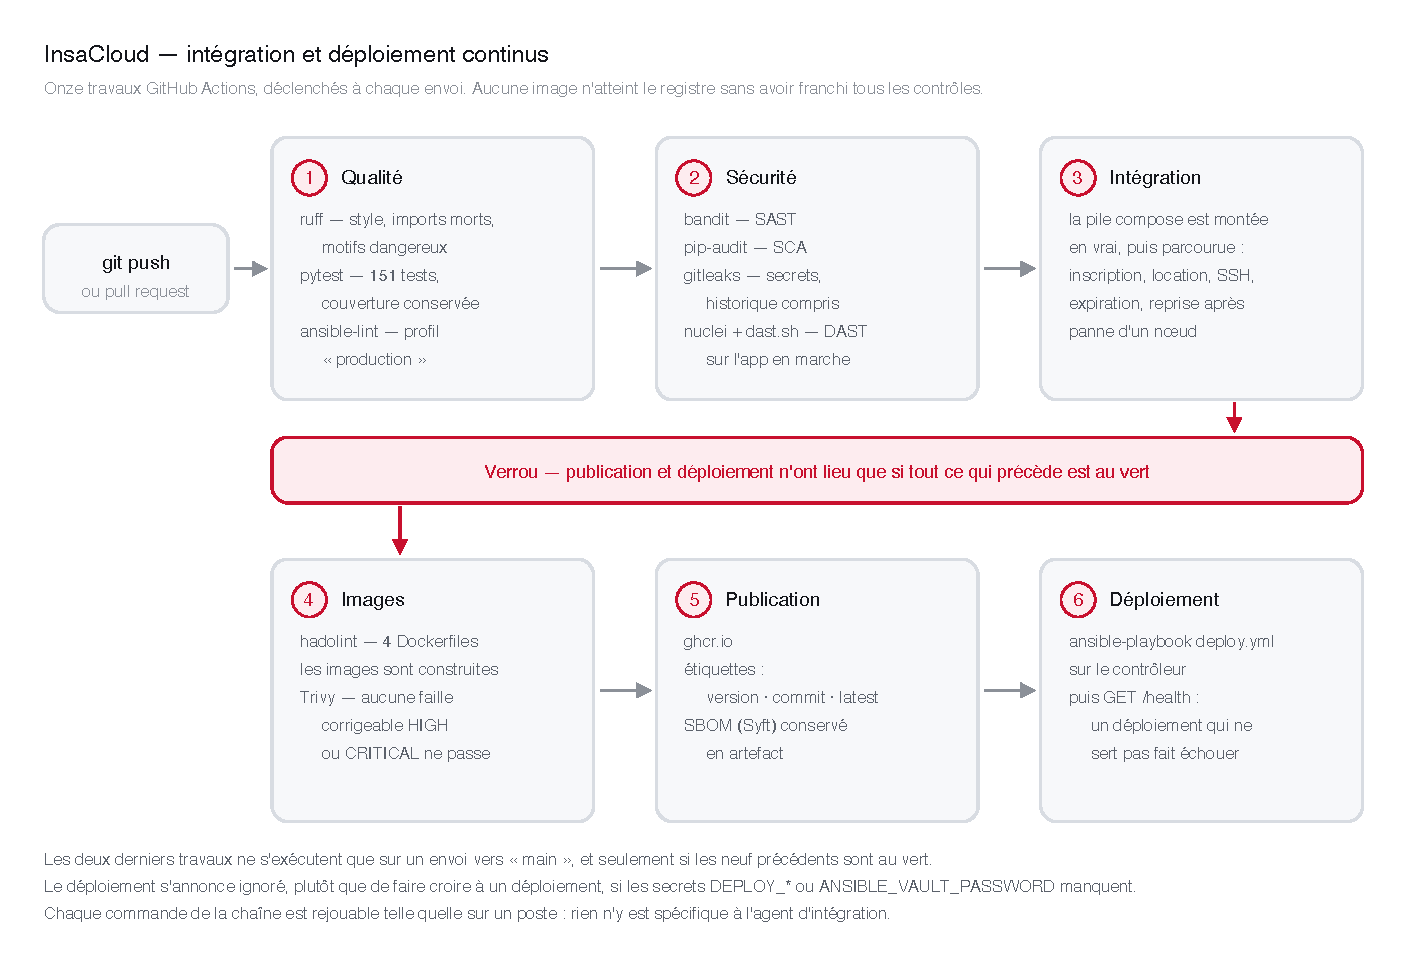
\includegraphics[width=\textwidth]{figures/chaine-ci-cd.pdf}
\caption{Les onze travaux et le verrou qui protège le registre.}
\end{figure}

\begin{center}
\small
\begin{tabularx}{\textwidth}{@{}llX@{}}
\toprule
\textbf{Travail} & \textbf{Outil} & \textbf{Ce qu'il attrape} \\
\midrule
Lint Python & \cmd{ruff} & imports morts, noms inconnus, motifs douteux \\
Tests & \cmd{pytest} & 169 cas, couverture conservée en artefact \\
SAST & \cmd{bandit} & injection, secrets en dur, appels système risqués \\
SCA & \cmd{pip-audit} & CVE des dépendances épinglées \\
Secrets & \cmd{gitleaks} & clés commises, y compris dans l'historique \\
DAST & \cmd{dast.sh} + \cmd{nuclei} & l'application en fonctionnement \\
Lint Ansible & \cmd{ansible-lint} & rôles, profil \cmd{production} \\
Images & \cmd{hadolint} + \cmd{Trivy} & 4 Dockerfiles, CVE des images \\
Intégration & \cmd{docker compose} & la pile démarre et une machine se loue \\
Publication & \cmd{Syft} + \cmd{ghcr.io} & SBOM conservé, images étiquetées \\
Déploiement & \cmd{ansible-playbook} & met à jour l'hôte puis interroge \cmd{/health} \\
\bottomrule
\end{tabularx}
\end{center}

\section{Le verrou}

Les deux derniers travaux ne s'exécutent que sur un envoi vers \cmd{main}, et
seulement si les neuf précédents sont au vert :

\begin{lstlisting}[language=yamlplus]
  publier-images:
    needs: [lint-python, tests-python, sast-python, sca-dependances, secrets,
            dast, lint-ansible, images-docker, integration]
    if: github.event_name == 'push' && github.ref == 'refs/heads/main'
\end{lstlisting}

\begin{retenir}
Sans \cmd{needs:}, GitHub Actions lance tous les travaux en parallèle --- et
publierait l'image pendant que les tests échouent. La dépendance explicite
est ce qui transforme une liste de contrôles en une véritable barrière.
\end{retenir}

\section{Trois incidents instructifs}

\paragraph{Nos images refusées par notre propre scan.} Le travail
\cmd{images-docker} refuse toute faille corrigeable de niveau HIGH ou
CRITICAL. Notre image utilisait \cmd{docker:28-cli}, qui traînait 163 failles
corrigeables liées à sa version de Go, plus des CVE OpenSSL héritées de la
base Debian.

La correction a tenu en deux gestes : passer à \cmd{docker:29-cli} (2 failles
au lieu de 163) et ajouter un \cmd{apt-get upgrade} pour OpenSSL. Le verrou
utilise par ailleurs \cmd{--ignore-unfixed} : refuser une faille sans correctif
disponible ne protégerait de rien et bloquerait tout.

\paragraph{Une dépendance qui n'existe pas pour la cible.} Le projet épinglait
SQLAlchemy 2.1.1, disponible sur notre poste. La cible de déploiement est
Ubuntu 22.04, qui fournit Python 3.10 --- pour lequel cette version n'a jamais
été publiée. Les tests passaient, le déploiement échouait.

\paragraph{Deux guillemets déséquilibrées.} Une erreur de syntaxe shell dans un
bloc \cmd{run:} ne se voit qu'au moment où l'étape s'exécute, parfois après dix
minutes de chaîne. Trois exécutions ont échoué ainsi. Nous avons ajouté un
contrôle qui extrait chaque bloc \cmd{run:}, neutralise les expressions
\cmd{\$\{\{ \}\}} et passe le tout à \cmd{bash -n} :

\begin{lstlisting}[language=yamlplus,caption={\fichier{.github/workflows/ci.yml} --- la chaîne vérifie sa propre syntaxe}]
      - name: Verifier la syntaxe shell de la chaine elle-meme
        run: |
          pip install --quiet pyyaml
          python3 .github/verifier-workflow.py
\end{lstlisting}

\begin{retenir}
Chaque fois qu'un défaut vous a coûté du temps, demandez-vous quel contrôle
automatique l'aurait attrapé --- puis ajoutez-le. Une chaîne d'intégration
n'est pas écrite d'un coup : elle se construit par sédimentation, un incident
après l'autre.
\end{retenir}

\section{Empêcher la documentation de vieillir}

Les schémas du dépôt sont engendrés par des scripts Python ; la chaîne les
régénère et refuse la moindre différence :

\begin{lstlisting}[language=yamlplus]
      - name: Verifier que les schemas du README sont a jour
        run: |
          python3 docs/schemas/tout.py
          git diff --exit-code -- docs/*.svg
\end{lstlisting}

\begin{piege}{Du texte à jour, des images périmées}
Ce garde-fou vient d'une erreur réelle. Le README avait été mis à jour ---
texte, chiffres, descriptions d'images --- mais les schémas SVG, eux,
montraient encore deux workers alors que le projet en comptait trois.

La moitié du contenu d'un README est visuelle. La traiter comme du texte, c'est
garantir qu'elle finira fausse.
\end{piege}

\chapter{Ce qu'on a trouvé en faisant tourner}

Les défauts qui suivent n'ont pas été trouvés en relisant le code, mais en le
faisant fonctionner : en déployant sur un cluster, en lançant la pile, en
lisant les journaux.

\begin{center}
\small
\begin{tabularx}{\textwidth}{@{}XX@{}}
\toprule
\textbf{Défaut} & \textbf{Garde-fou ajouté} \\
\midrule
Le Faucheur détruisait sa propre plateforme : il reconnaissait les machines
à leur préfixe de nom &
Identité par étiquette Docker, plus jamais par nom ; un test le vérifie \\
\addlinespace
Deux déploiements sur un même démon se supprimaient mutuellement leurs
conteneurs &
Un second label délimite le déploiement \\
\addlinespace
Le mot de passe de la base journalisé en clair au démarrage du Faucheur &
Toute URL passe par une fonction de masquage \\
\addlinespace
Une dépendance épinglée inexistante pour le Python de la cible &
La chaîne installe exactement \cmd{requirements.txt} sur la cible réelle \\
\addlinespace
Des distributions proposées sans image construite &
Le catalogue interroge Docker avant d'afficher un choix \\
\addlinespace
Course au démarrage entre les quatre processus Gunicorn &
Création tolérante à la concurrence, et \cmd{--preload} \\
\addlinespace
Images refusées par notre propre scan Trivy &
Base plus récente, \cmd{apt-get upgrade}, \cmd{--ignore-unfixed} \\
\addlinespace
Deux guillemets déséquilibrées dans la chaîne elle-même &
Un contrôle de syntaxe shell de tous les blocs \cmd{run:} \\
\addlinespace
Le mot de passe root lisible dans le cookie de session &
Seul l'identifiant transite ; le secret est relu chiffré en base \\
\addlinespace
Les schémas du README figés sur une ancienne architecture &
La chaîne régénère les SVG et refuse toute différence \\
\bottomrule
\end{tabularx}
\end{center}

\begin{retenir}
Dix défauts, dix garde-fous. C'est la différence entre « on a corrigé » et
« cela ne peut plus revenir ». Corriger sans ajouter de contrôle, c'est
accepter de recommencer.
\end{retenir}

\section{Ce qui a été vérifié sur un cluster réel}

\begin{itemize}
\item \textbf{Déploiement complet} : \cmd{failed=0} sur les quatre nœuds.
\item \textbf{Idempotence} : second passage à \cmd{changed=0} sur les quatre.
\item \textbf{Inscription spontanée} : les trois agents se sont enregistrés
  seuls, aucune adresse de worker n'étant écrite côté contrôleur.
\item \textbf{Parcours utilisateur} : inscription, location, accès ; le
  conteneur est bien créé sur le nœud le moins chargé.
\item \textbf{Durcissement effectif} : \cmd{docker inspect} confirme
  \cmd{restart=always}, les limites mémoire, \cmd{pids-limit},
  \cmd{cap-drop ALL} et \cmd{no-new-privileges}.
\item \textbf{Conservation de l'état} : après redémarrage du démon Docker
  \emph{puis} du nœud entier, la machine et le travail de l'utilisateur sont
  intacts.
\item \textbf{Faucheur} : une location d'une minute détruite 49 secondes après
  son expiration.
\item \textbf{Reprise sur panne} : le scénario de l'énoncé joué tel quel.
\item \textbf{Analyse dynamique} : 18 contrôles sur l'application en
  fonctionnement, tous réussis.
\end{itemize}
